\documentclass[12pt]{article}
\usepackage[utf8]{inputenc}
\usepackage[brazil]{babel}
\usepackage[margin = 1in]{geometry}
\usepackage{graphicx}
\usepackage{subfigure}
\usepackage{minted}
\usepackage{indentfirst}
\usepackage{float}
\usepackage{multirow}
\usepackage{textcomp}


\begin{document}

    
\begin{titlepage}
 \vfill
  \begin{center}
   {\large \textbf{UNIVERSIDADE FEDERAL DO PARANÁ \\ SETOR DE TECNOLOGIA \\ DEPARTAMENTO DE ENGENHARIA ELÉTRICA}} \\[5cm]

  {\large {Marco Antonio Rios  GRR20133243 \\ Wendeurick Silverio GRR20134722} }\\[4cm]


   {\Large \textbf{Projetos de Sistemas Digitais em PLD - TE087} \\ Laboratório 7}\\[6cm]
    \vfill

    \vspace{2cm}

    \large \textbf{Curitiba}

    \large \textbf{19 de maio de 2016}

      \end{center}
\end{titlepage}

\clearpage
%\tableofcontents    
%\clearpage

\section{Desafio A+}
O desafio ''A+'' propõe o projeto de um cronômetro digital, com funções pausa e reset, utilizando os 4 displays de 7 segmentos do kit NEXYS2. Ademais, o projeto deve ter a opção para alternar entre ''minutos-segundos'' e ''horas-minutos'', através de uma chave.

\subsection{Implementação}
O circuito tem como base a unidade contadora de milissegundo, que é utilizada tanto para os valores do cronômetro quanto para a taxa de atualização dos displays.

O tempo de cadência para os display é de 1ms por dígito, ou seja 1/(4x1ms) = 250fps, que é superior à taxa da percepção do olho humano. Assim, os números podem ser vistos como se todos os displays estivessem acesos ao mesmo tempo.

Buscou-se evitar o uso de operações como divisão e módulo, devido ao elevado custo operacional. Assim, a atualização entre unidade-de-segundo\textrightarrow dezena-de-segundo\textrightarrow unidade-de-minutos\textrightarrow [...] é feita através de comparações \emph{if}.

Abaixo, os códigos \emph{VHDL} e o mapeamento das entradas e saídas para o kit Nexys2.

\subsubsection{cronometro.vhd}
\inputminted{vhdl}{cronometro.vhd}

\subsubsection{display7seg.vhd}
\inputminted{vhdl}{display7seg.vhd}

\subsubsection{millis.vhd}
\inputminted{vhdl}{millis.vhd}

\subsubsection{desafio1\_pins.vhd}
\inputminted{vhdl}{cronometro_pins.ucf}

\subsection{Simulação}

Abaixo, o código \emph{VHDL} do Testbench.

\inputminted{vhdl}{cronometro_tb.vhd}

\clearpage

Apenas para fins de visualização na simulação, diminuíram-se os ciclos de contagem para que houvesse mudança dos valores num intervalo de tempo menor, tendo em vista que a implementação foi projetada para operar a 50MHz e, para que houvesse uma única alteração apenas no dígito de segundos, seria necessário simular 50.000.000 pontos (o que gera um custo computacional relativamente grande). A imagem abaixo apresenta o instante em que o cronômetro marcava 16:39.

\begin{figure}[!h]
    \centering
    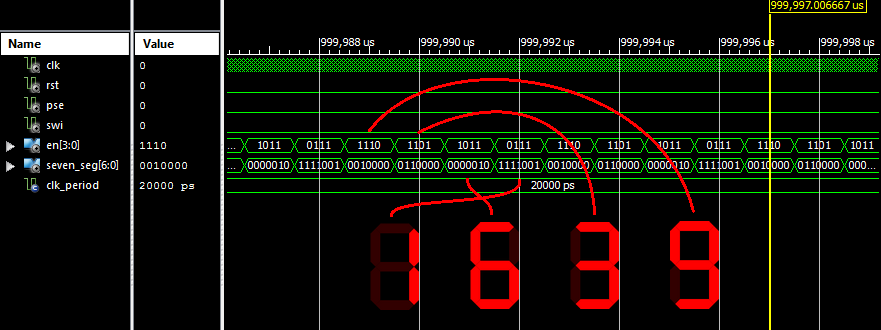
\includegraphics[width=1.0\textwidth]{tb.png}
    \caption{Testbench do cronômetro.}
\end{figure}

\end{document}
